\documentclass[main]{subfiles}
\begin{document}
\chapter{8の字を走行}

これは講義資料「第2回 ロボットの動かし方と基本的な動作」内の課題です。

\section{課題概要}
なおこの実験ではセンサを利用しないため、周囲に何もない場所で開始する必要がある。

\section{解法}

\begin{figure}[H]
	\begin{minipage}{0.5\hsize}
		\setlength{\parindent}{1\Cwd}
		二つの円を描くように走行させるにあたって
		円を切り替えるタイミングに注意する必要がある。
		先に反時計回りに上の円から描いていくのだが、
		単純に原点に近付いたタイミングで下の円の描画に切り替える実装をすると
		開始のタイミングとの区別がつかず下の円のみ描画されてしまう。

		そこで右図のように(1,0), (0,0), (-1,0)の3点に達した
		(正確には3点の半径1cm以内に入った)時点で
		命令が切り替わるように設計した。以下に命令列を書き下した。

		\begin{itemize}
			\item (0,1)に到達するまで上の円を描く
			\item (0,0)に到達するまで上の円を描く
			\item (0,-1)に到達するまで下の円を描く
			\item (0,0)に到達するまで下の円を描く
		\end{itemize}
	\end{minipage}
	\begin{minipage}{0.5\hsize}
		\begin{figure}[H]
			\centering
			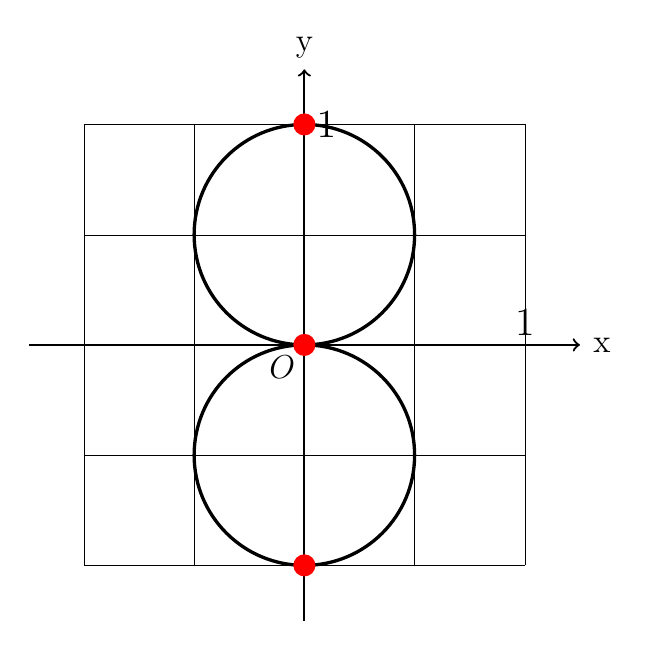
\begin{tikzpicture}[scale=1.4]
				\draw [ultra thin] (-2,-2) grid (2,2);
				\draw [thick,->] (-2.5,0) -- (2.5,0);
				\draw [thick,->] (0,-2.5) -- (0,2.5);
				\draw [very thick] (0,1) circle [x radius=1, y radius=1];
				\draw [very thick] (0,-1) circle [x radius=1, y radius=1];
				\node at (-0.2,-0.2) {\large $O$};
				\node at (2.7,0) {\large x};
				\node at (0,2.7) {\large y};
				\node at (0.2,2) {\Large $1$};
				\node at (2,0.2) {\Large $1$};

				\fill [red] (0,-2) circle [x radius=0.1, y radius=0.1];
				\fill [red] (0,0) circle [x radius=0.1, y radius=0.1];
				\fill [red] (0,2) circle [x radius=0.1, y radius=0.1];
			\end{tikzpicture}
			\caption{原点を出発して8の字を描くように進む}
		\end{figure}
	\end{minipage}
\end{figure}

\section{結果}
\begin{figure}[H]
	\centering
	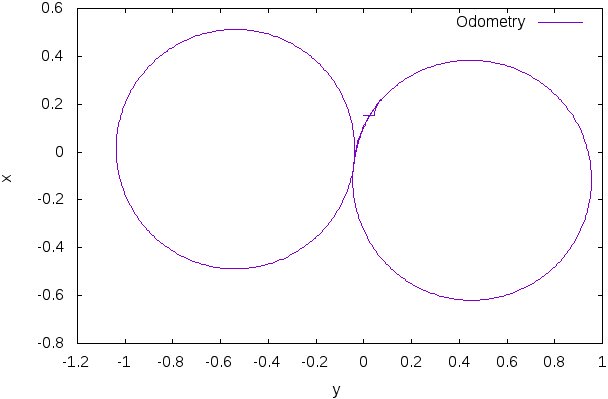
\includegraphics[width=8cm]{img/eight.png}
	\caption{8の字走行のオドメトリ}
\end{figure}

\section{考察}


\chapter{前方1m以内に障害物を見つけたら停止}

これは講義資料「第3回 測域センサの使い方」の課題です。

\section{課題概要}
\section{解法}

\section{結果}
\begin{figure}[H]
	\centering
	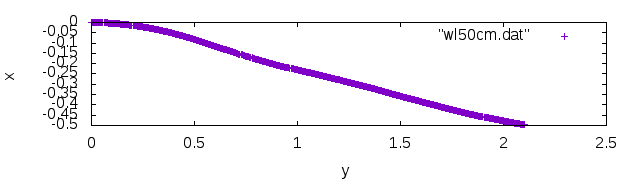
\includegraphics[width=15cm]{img/wl50cm.png}
\end{figure}
小刻みに調整が働いて壁と並行する線上を走行できていることがわかる。

\section{考察}


\end{document}
